\documentclass[a4paper]{article}

%% Language and font encodings
\usepackage[french]{babel}
\usepackage[utf8x]{inputenc}
\usepackage[T1]{fontenc}

%% Sets page size and margins
\usepackage[a4paper,top=3cm,bottom=3cm,left=2cm,right=2cm,marginparwidth=2cm]{geometry}

%% Useful packages
\usepackage{amsmath}
\usepackage{graphicx}
\usepackage[colorinlistoftodos]{todonotes}
\PassOptionsToPackage{hyphens}{url}
\usepackage[colorlinks=true, allcolors=black]{hyperref}
\usepackage{fourier-orns}
\usepackage{titlesec}
\usepackage{fancyhdr}
\usepackage{fancyvrb}
\usepackage{float}
\pagestyle{fancy} 
\setcounter{tocdepth}{5}

%% Tikz stuff
\usepackage{tikz}
\usetikzlibrary{calc, arrows, patterns}
\tikzstyle{incolore} = [rectangle, rounded corners, draw=black, minimum height=1cm, minimum width=3cm, text width=3cm, text centered]
\tikzstyle{field} = [rectangle,, draw=black, minimum height=1cm, minimum width=4cm, text width=3cm, text centered]

%% Pour les exemples
\usepackage{mdframed}
\newmdenv[topline=false, bottomline=false, rightline=false, skipabove=3pt, skipbelow=3pt]{example}

\usepackage{libertine}
\newcommand{\hsp}{\hspace{20pt}}
\newcommand{\HRule}{\rule{\linewidth}{0.5mm}}

\renewcommand{\headrulewidth}{1pt}
\fancyhead[C]{}
\fancyhead[L]{}
\fancyhead[R]{\footnotesize{\leftmark}}

\renewcommand{\footrulewidth}{1pt}
\fancyfoot[C]{}
\fancyhead[L]{}
\fancyfoot[R]{\thepage}

\definecolor{Zgris}{rgb}{0.87,0.85,0.85}

\usepackage{eso-pic,graphicx}
\usepackage{xcolor}
\newcommand{\bgimg}[1]
{
    \AddToShipoutPicture
    {
        \put(\LenToUnit{0 cm},\LenToUnit{0 cm})
        {
            \includegraphics[width=\paperwidth,height=\paperheight]{#1}
        }
    }
}

\usepackage{xcolor}
\usepackage{listings}

\definecolor{mGreen}{rgb}{0,0.6,0}

\lstdefinestyle{CStyle}{
    commentstyle=\color{mGreen},
    keywordstyle=\color{red},
    numberstyle=\color{gray},
    stringstyle=\color{purple},
    frame=single,
    escapeinside={\%*}{*)},
    breakatwhitespace=false,
    breaklines=true,
    captionpos=b,
    keepspaces=true,
    numbers=left,
    showspaces=false,
    showstringspaces=false,
    showtabs=false,
    tabsize=2,
    language=C
}

\begin{document}





\begin{titlepage}
    \begin{sffamily}
        \begin{center}

            
\includegraphics[width=5cm]{images/LogoHenallux.PNG}~\\[1.5cm]
            \textsc{\Large Rapport de projet}\\[1.5cm]

            \HRule \\[0.4cm]
            { \huge \bfseries Implémentation d'un IDS \\[0.4cm] }
            \HRule \\[2cm]

            \begin{minipage}{0.4\textwidth}
                \begin{flushleft} \large
                    Grégoire Roumache\\
                    Florian Fichet\\
                \end{flushleft}
            \end{minipage}
            \begin{minipage}{0.55\textwidth}
                \begin{flushright} \large
                    Développement -- Sécurité des systèmes\\
                    Deuxième année, groupe C-2 \\
                    Année académique 2020-2021\\
                \end{flushright}
            \end{minipage}
            \vfill

            {\large 3 Janvier 2021}

        \end{center}
    \end{sffamily}
\end{titlepage}

\let\cleardoublepage\clearpage










\section{Introduction}



Pour le cours de Développement, nous avons dû implémenter un IDS (Intrusion Detection System) qui analyse le trafic qui passe par une interface réseau de la machine. Il permet de détecter des activités suspectes en fonction d'un certain nombre de règles données au préalable. En cas d'anomalie, le programme peut alerter l'utilisateur en la signalant dans les logs du système.

Nous nous sommes organisés en utilisant la plateforme github, comme recommandé, et voici le lien vers notre répertoire: 
\begin{center}
    {\small \url{https://github.com/groumache/Intrusion-Detection-System}}
\end{center}










\section{Organisation du travail et configuration des outils}





\subsection{Les issues sur github}



Les issues sont utilisées pour s'organiser et garder une trace des tâches, des améliorations et des bugs dans un projet sur github.
\begin{figure}[H]
    \centering
    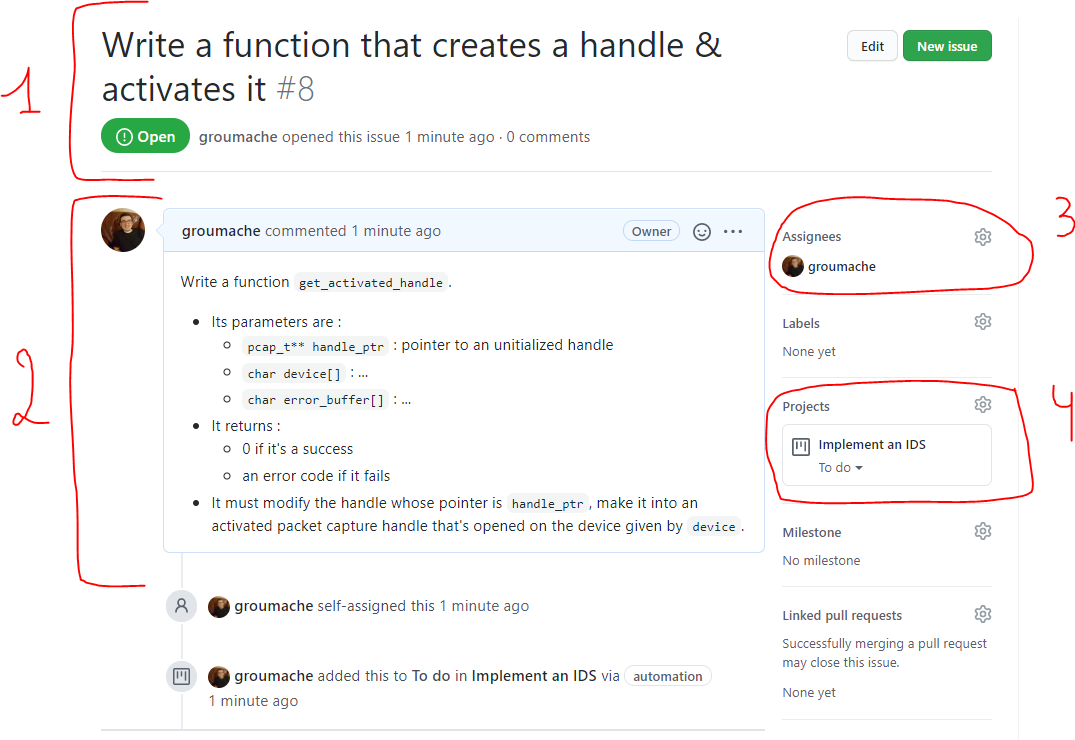
\includegraphics[width=0.99\linewidth]{../markdown-explanations/images/issue-1.PNG}
    \caption{Une issue sur github}
    \label{fig:issue01}
\end{figure}
Explication de la figure \ref{fig:issue01}:
\begin{enumerate}
    \item Titre de l'issue.
    \item Explication/description de l'issue.
    \item On peut attribuer une issue à des personnes qui seront responsables pour résoudre l'issue.
    \item Le projet dans lequel l'issue va apparaître.
\end{enumerate}





\subsection{Utilisation du kanban sur github}



Comme nous l'avons précisé dans l'introduction, nous nous sommes organisés en utilisant github. Nous n'avons pas seulement mis le code sur github mais aussi utilisé le tableau kanban avec 4 sections:
\begin{enumerate}
    \item \textbf{Ideas}: un endroit pour ajouter des notes/issues qui dépassent les exigences du projet.
    \item \textbf{To do}: un endroit où les issues sont placées quand elles sont créées (correspond aux critères minimum de réussite).
    \item \textbf{In progress}: l'endroit où les issues vont quand on travaille dessus.
    \item \textbf{Done}: là où les issues vont quand elles sont fermées ou la pull request liée a été fusionnée.
\end{enumerate}
\begin{figure}[H]
    \centering
    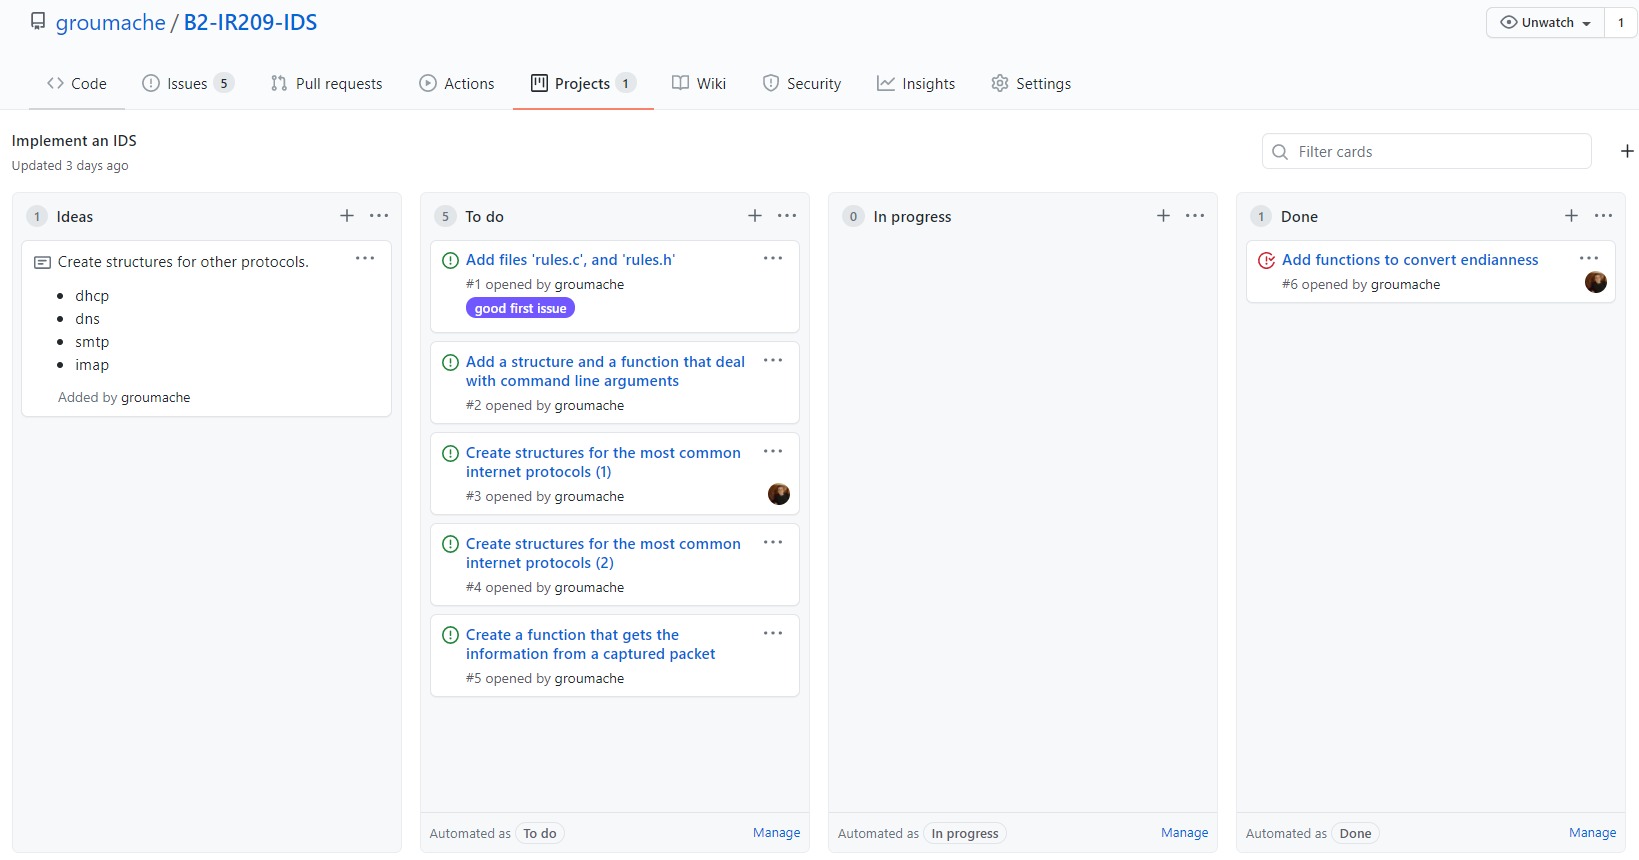
\includegraphics[width=0.99\linewidth]{../markdown-explanations/images/project-1.PNG}
    \caption{Kanban sur github}
\end{figure}

Sur le schéma de la figure \ref{fig:networkgraph}, on voit le network graph. Cette image illustre bien comment nous avons travaillé, c-à-d en créant des nouvelles branches à chaque fois que nous avons eu besoin de résoudre une issue. Une fois que le code a été ajouté, nous avons fait des pull requests pour fusionner les branches.
\begin{figure}[H]
    \centering
    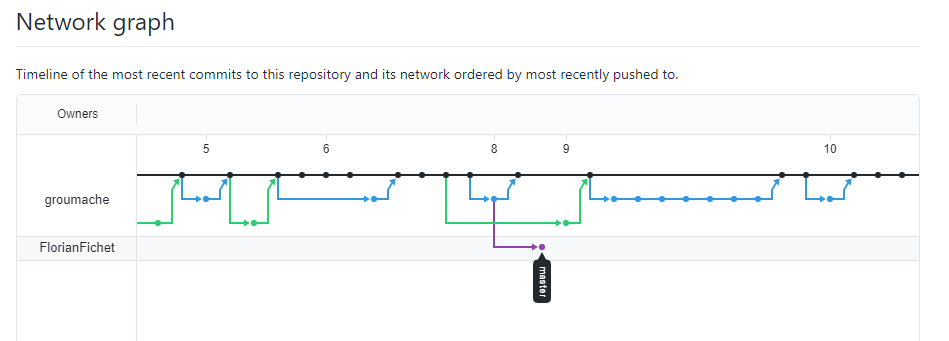
\includegraphics[width=0.99\linewidth]{../markdown-explanations/images/project-2.PNG}
    \caption{Network graph montrant les commits et comment les branches se rejoignent}
    \label{fig:networkgraph}
\end{figure}





\subsection{Configuration du debugger}



Les fichiers de configurations sont présentés sur les figures \ref{fig:debugconfig1} et \ref{fig:debugconfig2}.
\begin{enumerate}
    \item Sur la figure \ref{fig:debugconfig1}, on voit le fichier \textit{tasks.json} où on configure la compilation du projet:
    \begin{itemize}
        \item on voit que le paramètre \textit{command} donne bien le compilateur gcc,
        \item les arguments sont précisés par le paramètre \textit{args}, ce sont ceux recommandés dans l'énoncé,
        \item si on combine le tout, c'est l'équivalent de la commande:
        \begin{center}
            \texttt{\small gcc -Wall -o ids main.c populate.c rules.c error.c -lpcap}
        \end{center}
    \end{itemize}
    \item Sur la figure \ref{fig:debugconfig2}, on voit le fichier \textit{launch.json}, il sert à configurer le lancement du programme:
    \begin{itemize}
        \item dans \textit{program}, on voit qu'on a bien précisé \textit{ids},
        \item et dans \textit{args}, on voit les arguments du programme.
        \item si on combine le tout, c'est l'équivalent de la commande:
        \begin{center}
            \texttt{\small ids -p -d eth1 -r ids.rules -n 10 -{}-print-logs -{}-print-all}
        \end{center}
    \end{itemize}
\end{enumerate}
Remarques:
\begin{itemize}
    \item Il faut lancer le programme avec des privilèges plus élevé que l'utilisateur standard. Pour réussir à faire cela, on peut lancer visual studio code avec ces mêmes privilèges.
    \item Les chemins des fichiers devront être modifiés si on clone le répertoire github sur une autre machine.
\end{itemize}
\begin{figure}[H]
    \centering
    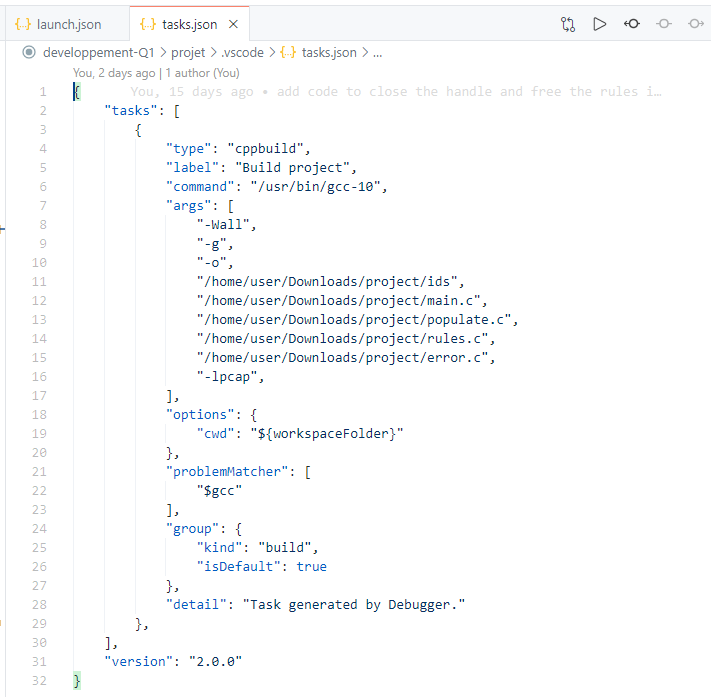
\includegraphics[width=0.85\linewidth]{images/task-json.PNG}
    \caption{Fichier de configuration du debugger, pour la compilation du programme}
    \label{fig:debugconfig1}
\end{figure}
\begin{figure}[H]
    \centering
    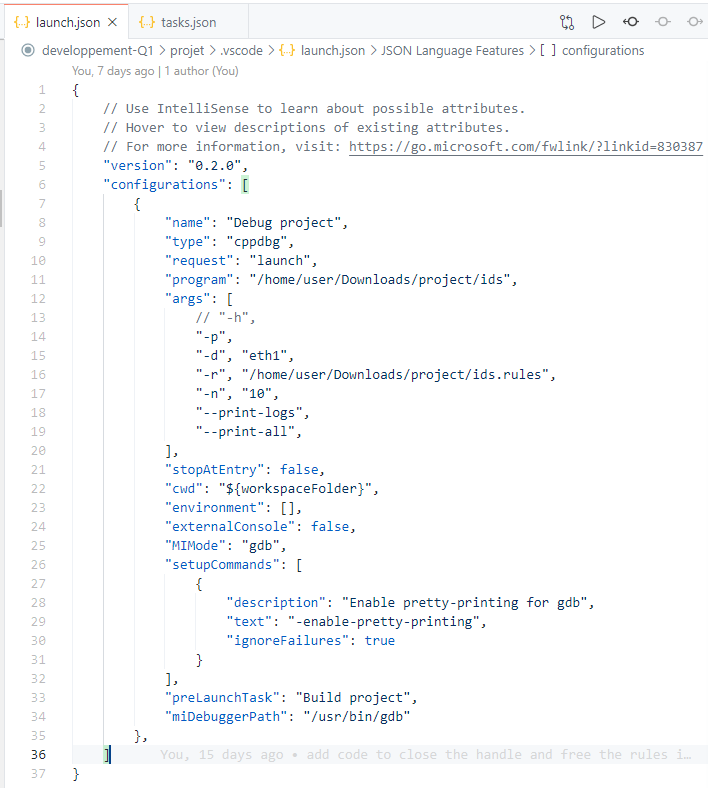
\includegraphics[width=0.85\linewidth]{images/launch-json.PNG}
    \caption{Fichiers de configuration du debugger, pour lancer le programme}
    \label{fig:debugconfig2}
\end{figure}





\subsection{Utilisation de valgrind}



Valgrind est un outil de programmation qui sert principalement à découvrir des fuites de mémoire. Par exemple, si nous allouons un bloc de mémoire dans le tas (heap) et que nous ne le libèrons pas, valgrind va nous rappeler à l'ordre et même nous dire à quelle ligne le bloc mémoire à été alloué (si le programme a été compilé avec un debug flag).

Lancement du programme avec valgrind (rappel: ids doit être lancé avec des privilèges):
{\small \begin{verbatim}
    valgrind --leak-check=full \
        --show-leak-kinds=all \
        --track-origins=yes \
        --verbose \
        ./ids
\end{verbatim}}

L'objectif est donc d'obtenir un résultat comme celui à la figure \ref{fig:valgrind}.

\begin{figure}[H]
    \centering
    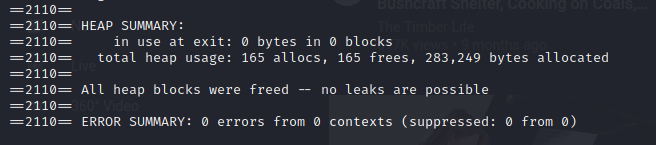
\includegraphics[width=0.75\linewidth]{../markdown-explanations/images/valgrind-01.PNG}
    \caption{Résultat de valgrind}
    \label{fig:valgrind}
\end{figure}





\subsection{Configuration du formatage automatique}



L'extension C/C++ de visual studio code nous permet de faire du formatage automatique de notre code comme illustré par la figure \ref{fig:formatting}. La configuration se fait au en suivant la syntaxe clang-format, voici celle que nous avons utilisé:

{\small\begin{verbatim}
{
    BasedOnStyle: Google,
    IndentWidth: 4,
    MaxEmptyLinesToKeep: 2,
    IndentPPDirectives: BeforeHash
}
\end{verbatim}}

\begin{figure}[H]
    \centering
    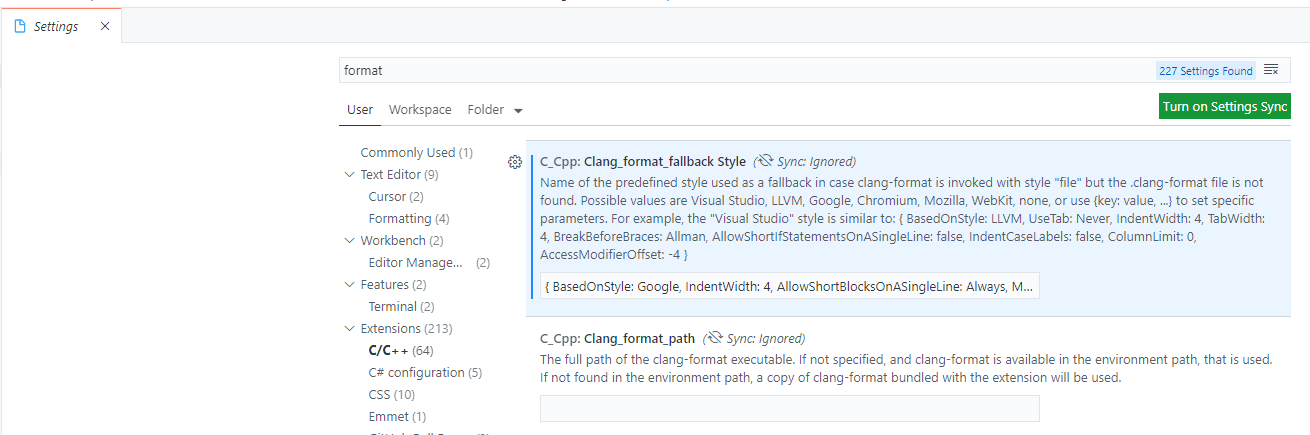
\includegraphics[width=0.99\linewidth]{../markdown-explanations/images/setup-04.PNG}
    \caption{Paramètre de formatage dans visual studio code}
    \label{fig:formatting}
\end{figure}










\section{Architecture du projet}





\subsection{Architecture du système}



Comme on peut voir sur la figure \ref{fig:archsys}, l'ids est divisé en quatre parties logiques.
\begin{enumerate}
    \item \textit{read\_rules}: cette partie est responsable d'extraire les règles du fichier pour les mettre dans les structures appropriées
    \item \textit{populate\_packet}: cette partie doit extraire le paquet pour le placer dans les structures appropriées
    \item \textit{main}: cette partie a 4 responsabilités:
    \begin{itemize}
        \item analyse les arguments du programme
        \item faire appel aux parties \textit{read\_rules}, et \textit{populate\_packet}
        \item vérifier si les packets correspondent aux règles
        \item si ils correspondent aux règles, elle doit écrire un message dans syslog
    \end{itemize}
\end{enumerate}

\begin{figure}[H]
    \centering
    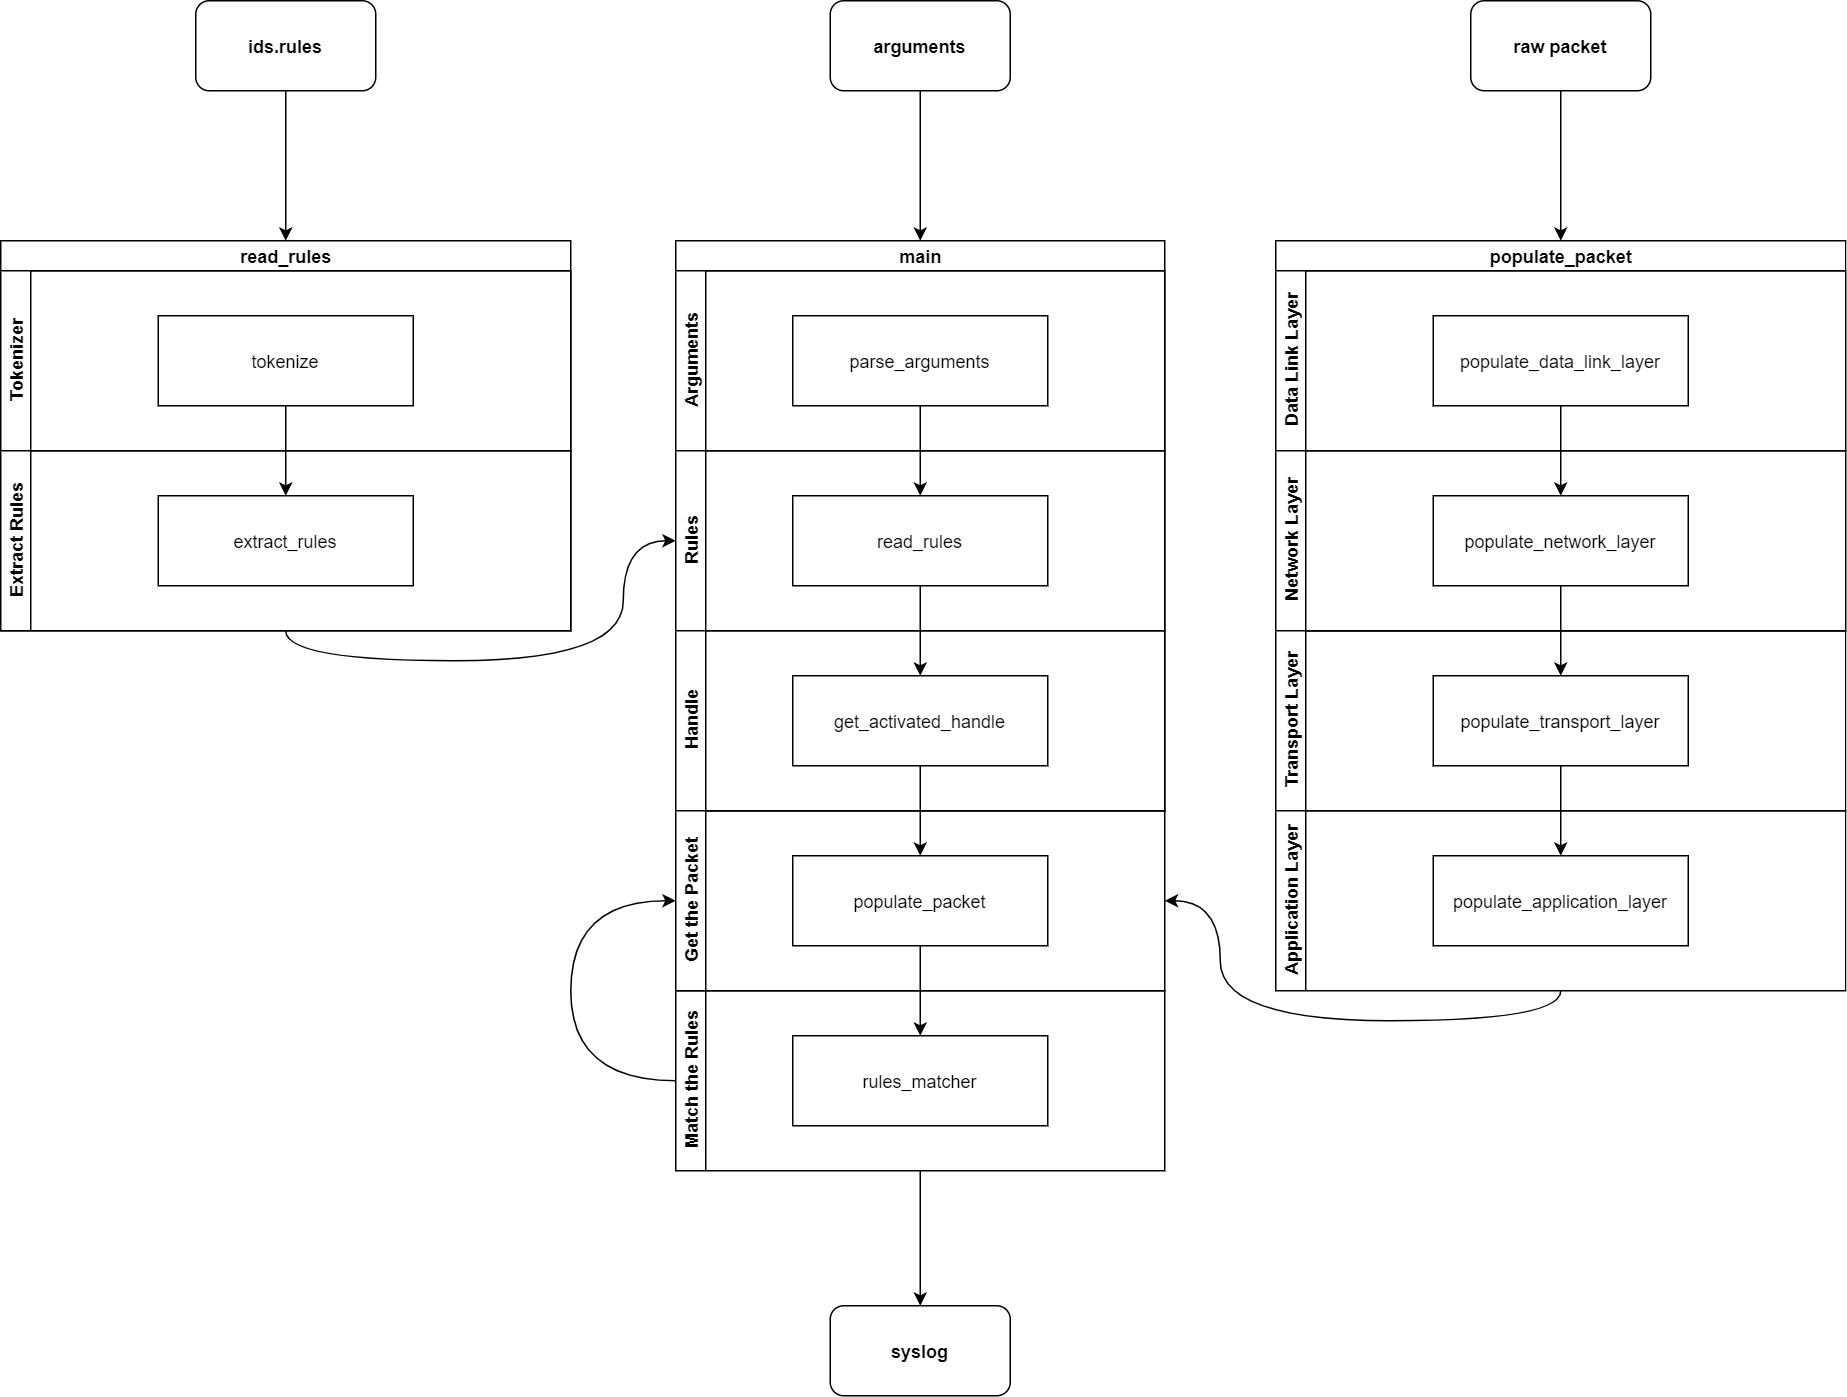
\includegraphics[width=0.99\linewidth]{../markdown-explanations/images/software-architecture-2.png}
    \caption{Architecture du système}
    \label{fig:archsys}
\end{figure}





\subsection{Structure du projet}



Pour mieux comprendre l'organisation du projet, on peut regarder la figure \ref{fig:structproj} sert à montrer quels fichiers sont inclus dans quels autres.

\begin{figure}[H]
    \centering
    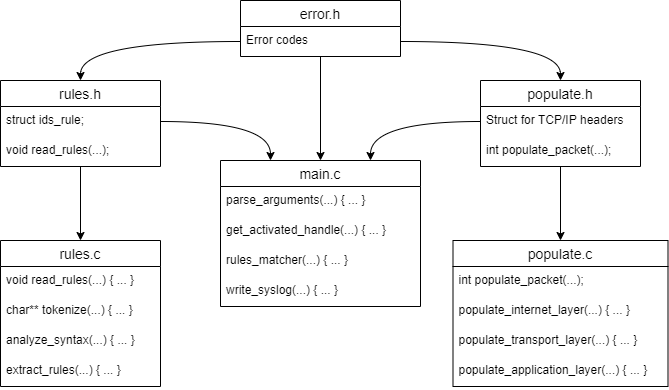
\includegraphics[width=0.90\linewidth]{../markdown-explanations/images/project-structure.png}
    \caption{Structure du projet}
    \label{fig:structproj}
\end{figure}










\section{Organisation générale du code}



Dans cette section, nous allons expliquer comment le code fonctionne de manière générale mais sans entrer dans le détail. Les choix d'implémentation spécifiques seront expliqués dans la section suivante (section \ref{sec:implspec}).





\subsection{Fichier \textit{populate.c}}



Les 3 fonctions de ce fichier qui ont leur définition dans le header \textit{populate.h} sont:
\begin{itemize}
    \item \textit{populate\_packet}, organise les informations à partir de la trame brute
    \item \textit{print\_packet\_headers}, affiche les headers des protocols utilisés dans le paquet
    \item \textit{print\_packet\_data}, affiche les données contenues dans le protocole de dernière couche (HTTP, TLS, TCP ou UDP)
\end{itemize}
La fonction la plus importante de ce fichier est évidemment la fonction \textit{populate\_packet} qui va appeler d'autres fonctions \textit{populate} comme représenté sur la figure \ref{fig:orgpopulate}.
\begin{figure}[H]
    \centering
    \begin{tikzpicture}

        \node (packet) [incolore] at (0,0) {\textit{populate packet}};

        \node (datalink) [incolore] at (-6,-2) {\textit{populate data link}};
        \node (network) [incolore] at (-2,-2) {\textit{populate network}};
        \node (transport) [incolore] at (2,-2) {\textit{populate transport}};
        \node (application) [incolore] at (6,-2) {\textit{populate application}};

        \node (tcp) [incolore] at (0,-4) {populate tcp};
        \node (udp) [incolore] at (4,-4) {populate udp};

        \draw[->] (packet) -- (datalink);
        \draw[->] (packet) -- (network);
        \draw[->] (packet) -- (transport);
        \draw[->] (packet) -- (application);

        \draw[->] (transport) -- (tcp);
        \draw[->] (transport) -- (udp);

    \end{tikzpicture}
    \caption{Organisation des fonctions \textit{populate}}
    \label{fig:orgpopulate}
\end{figure}





\subsection{Fichier \textit{rules.c}}



Les fonctions de ce fichier qui ont leur définition dans le header \textit{rules.h} sont:
\begin{itemize}
    \item \textit{read\_rules}
    \item \textit{free\_rules}
\end{itemize}
La fonction la plus importante de ce fichier est \textit{read\_rules} qui va faire la tokenisation du fichier de règles (voir section \ref{subsec:tokens} pour des explications sur les tokens) puis en extraire les règles, ceci est illustré par la figure \ref{fig:orgrules}.
\begin{figure}[H]
    \centering
    \begin{tikzpicture}

        \node (read) [incolore] at (0,0) {\textit{read rules}};

        \node (token) [incolore] at (-4,-2) {\textit{tokenize rules}};
        \node (extract) [incolore] at (4,-2) {\textit{extract rules}};

        \node (action) [incolore] at (-6,-4) {\textit{get action}};
        \node (protocol) [incolore] at (-2,-4) {\textit{get protocol}};
        \node (dots) [incolore] at (2,-4) {\textit{...}};
        \node (options) [incolore] at (6,-4) {\textit{get options}};

        \node (settings) [incolore] at (6,-6) {\textit{get option settings}};

        \draw[->] (read) -- (token);
        \draw[->] (read) -- (extract);

        \draw[->] (extract) -- (action);
        \draw[->] (extract) -- (protocol);
        \draw[->] (extract) -- (dots);
        \draw[->] (extract) -- (options);

        \draw[->] (options) -- (settings);

    \end{tikzpicture}
    \caption{Organisation des fonctions utilisées pour extraire les règles}
    \label{fig:orgrules}
\end{figure}

Les fonctions pour obtenir les IPs et les ports sont plus compliquées parce que nous avons suivi le format de règle de \textit{surricata} \cite{2}. Ces formats sont représentés sur les figures \ref{fig:formatip} et \ref{fig:formatport}.
\begin{figure}[H]
    \centering
    \begin{tabular}{|c|c|} \hline
        \textbf{Opérateur} & \textbf{Description} \\ \hline
        ../.. & range d'IPs (notation CIDR) \\
        ! & exception/négation \\
        $[$.., ..$]$ & groupement \\ \hline
    \end{tabular}
    \caption{Format d'IP acceptable dans le fichier de règles}
    \label{fig:formatip}
\end{figure}
\begin{figure}[H]
    \centering
    \begin{tabular}{|c|c|} \hline
        \textbf{Opérateur} & \textbf{Description} \\ \hline
        : & range de ports \\
        ! & exception/négation \\
        $[$.., ..$]$ & groupement \\ \hline
    \end{tabular}
    \caption{Format de port acceptable dans le fichier de règles}
    \label{fig:formatport}
\end{figure}





\subsection{Fichier \textit{main.c}}



Il y a deux structures dans \textit{main.c}:
\begin{itemize}
    \item \textit{IdsArguments}, sert à stocker les paramètres donnés en ligne de commande à l'IDS,
    \item \textit{UserArgsPacketHandler}, sert à stocker des paramètres pour la fonction \textit{packet\_handler} tels que les règles du programme et les arguments de l'IDS lui-même.
\end{itemize}
Il y a aussi quelques fonctions à noter dans le fichier \textit{main.c}:
\begin{itemize}
    \item \textit{main}, c'est le point d'entrée du programme, elle va appeler les autres fonctions de l'ids,
    \item \textit{packet\_handler}, fonction appellée par \textit{pacp\_loop} quand un paquet est capturé, elle doit utiliser les fonctions \textit{populate\_packet} et \textit{rules\_matcher} pour vérifier si le paquet correspond à une règle,
    \item \textit{rules\_matcher}, vérifie si le paquet correspond à une règle,
    \item \textit{parse\_arguments}, analyse les arguments donnés en ligne de commande,
    \item \textit{write\_syslog}, écrit un message dans syslog.
\end{itemize}





\subsection{Détection de l’encryption du payload}



Dans la section \textit{critères minimum de réussite} de l'énoncé, il nous est demandé de pouvoir faire la \textit{détection de l'encryption du payload}. Cependant, c'est une tâche difficile si on doit le faire pour tous les paquets. D'autant plus que des données compressées ressemblent souvent à des données cryptées \cite{3}.

Ce que nous avons décidé de faire est donc de laisser l'utilisateur écrire des règles pour des protocoles de chiffrement des données comme TLS qui seront détectés en fonction du port (source ou destination) utilisé. Notre implémentation différe en deux points de la recommendation donnée (figure \ref{fig:tls01}):
\begin{enumerate}
    \item Nous ne cherchons pas à détecter la poignée de main TLS sur le port 443 car c'est le seul protocole qui utilise ce port \cite{5}. Si un paquet est transmis avec ce port, il est directement signalé en tant que paquet utilisant TLS.
    \item Nous ne gardons pas trace de la communication en utilisant les numéros de séquence de paquet TCP mais nous utilisons uniquement le port utilisé. Ceci découle du point précédent, c-à-d qu'un paquet est signalé en fonction de son port. Et puisqu'une communication TCP/UDP est identifiée en utilisant ces ports, elle ne peut pas les changer \cite{4}. Il n'y a pas non plus besoin de garder une trace de la communication avec une variable (le port utilisé est suffisant pour identifier la communication).
\end{enumerate}
Il y a deux problèmes à cette approche:
\begin{itemize}
    \item Le protocole TLS peut être utilisé sur d'autres ports mais sa détection devient ardue puisqu'il faut dès lors chercher la présence du header TLS dans tous les paquets peut importe leur port. Ceci augmente aussi le risque de signalement de paquets n'utilisant pas le TLS.
    \item Du trafic légitime pourrait passer sur un port réservé au protocole TLS. Cependant, il y a peu de chance que cela arrive puisque le port est réservé.
\end{itemize}
En résumé:
\[
    \left.\begin{aligned}
        &\text{le trafic non-crypté ne doit pas passer sur le port 443}\\
        &\text{le trafic crypté passant par d'autres ports est trop difficile à vérifier}
    \end{aligned}\right\} \text{nous ne vérifions que le port 443}
\]

\begin{figure}[H]
    \centering
    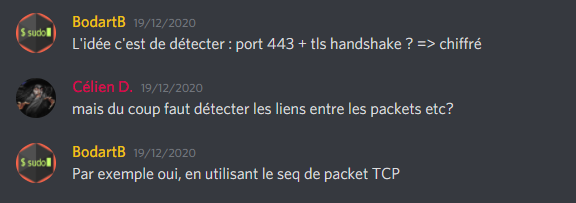
\includegraphics[width=0.75\linewidth]{images/tls-01.PNG}
    \caption{Recommendation pour détecter et garder trace des paquets chiffrés}
    \label{fig:tls01}
\end{figure}










\section{Choix d'implémentation et problèmes rencontrés} \label{sec:implspec}





\subsection{Tokens} \label{subsec:tokens}



La tokenisation c'est la séparation d'un texte en plus petites unités appelées tokens (comme illustré sur la figure \ref{fig:tokenization}). L'utilité de la tokenisation dans ce projet est que l'on a séparé deux choses:
\begin{itemize}
    \item le traitement des informations contenues dans le texte,
    \item et la recherche des informations.
\end{itemize}
Ainsi, la fonction \textit{extract\_rules} (appellée par \textit{read\_rules} après la tokenisation) ne doit pas chercher où commence et finit un protocole dans le fichier de règle puisque ça a été pris en charge par la fonction \textit{tokenize\_rules}, elle est seulement responsable d'extraire l'information du token.

\begin{figure}[H]
    \centering
    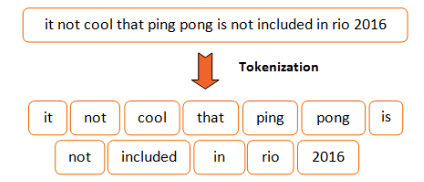
\includegraphics[width=0.65\linewidth]{images/tokenization.png}
    \caption{Illustration de la tokenisation \cite{6}}
    \label{fig:tokenization}
\end{figure}

Nous avons mis ci-dessous la fonction \textit{extract\_rules} qui extrait les règles des tokens et les met dans les structures \textit{Rule}. La variable \textit{i} est utilisée pour itérer sur les tokens. Cependant il y a un problème: si une IP, par exemple, est en fait une liste d'IP écrite sur plusieurs tokens (voir figure \ref{fig:formatip} sur les formats d'IP), de combien doit-on incrémenter la variable \textit{i} ?

Pour résoudre ce problème, le pointeur de la variable \textit{i} est passé en paramètre des fonctions qui servent à obtenir la règle (comme \textit{get\_rule\_action} ou \textit{get\_rule\_source\_ip}). Ce sont désormais ces fonctions qui sont responsables d'incrémenter \textit{i}. Ainsi, si une liste d'IP source prend vingt tokens, la fonction \textit{get\_rule\_source\_ip} devra incrémenter \textit{i} de vingt.
\begin{lstlisting}[style=CStyle]
void extract_rules(Rule **rules_ptr, int *nb_rules, Tokens *tokens) {
    int i = 0;
    while (i < tokens->nb_tokens) {
        // add an empty rule to the list
        ...

        // initialize the rule
        ...

        // get the rule
        get_rule_action(rule, tokens, &i);
        get_rule_protocol(rule, tokens, &i);
        get_rule_source_ip(rule, tokens, &i);
        get_rule_source_port(rule, tokens, &i);
        get_rule_direction(rule, tokens, &i);
        get_rule_destination_ip(rule, tokens, &i);
        get_rule_destination_port(rule, tokens, &i);
        get_rule_options(rule, tokens, &i);

        // NOTE: no need to increase i (i++) as it is incremented in the
        // functions used above
    }
}
\end{lstlisting}





\subsection{Structures de données dynamiques}



Dans ce projet, nous nous sommes souvent retouvés face à des quantités inconnues. Par exemple, combien de règles allons nous avoir dans le fichier de règles ? Pour résoudre ce problème, nous avons ajouter des fonctions, telle que \textit{increase\_nb\_rules} ci-dessous. Elles sont chargées de ré-allouer la mémoire afin que la "liste" d'éléments puisse grandir dynamiquement en fonction des besoins du programme.

\begin{lstlisting}[style=CStyle]
void increase_nb_rules(Rule **rules_ptr, int *nb_rules) {
    (*nb_rules)++;
    (*rules_ptr) = realloc((*rules_ptr), (*nb_rules) * sizeof(Rule));
}
\end{lstlisting}





\subsection{Problèmes d'endianness} \label{subsec:probendianness}



Il y a deux manières de représenter un nombre qui occupe plusieurs octets (voir figure \ref{fig:endianness}):
\begin{itemize}
    \item placer les octets de poids fort dans l'ordre des adresses (big endian),
    \item ou bien les placer dans l'ordre inverse des adresses (little endian).
\end{itemize}
\begin{figure}[H]
    \centering
    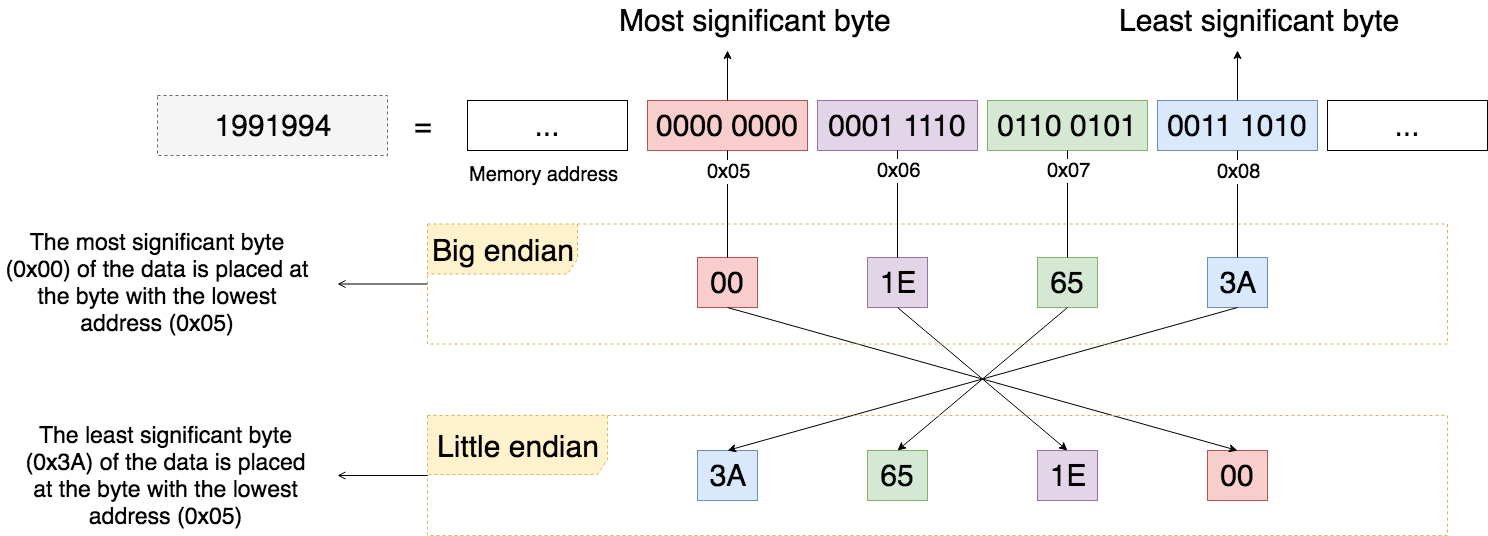
\includegraphics[width=0.90\linewidth]{images/Endian-Overview.png}
    \caption{Illustration des deux types d'endianness \cite{7}}
    \label{fig:endianness}
\end{figure}

Le problème vient que les protocoles internet sont codés en big endian, alors que l'architecture x86 code les nombres avec le format little endian. Cela pose problème quand, par exemple, on reçoit le type de protocole dans une trame ethernet. Si on reçoit un paquet IPv4, on aura:
\begin{itemize}
    \item 0x0800 = 2048, en big endian,
    \item qui sera interprété comme étant: 0x0008 = 8, en little endian !
\end{itemize}
Nous devons donc changer l'ordre des octets pour pouvoir interpréter correctement les informations reçues. Ceci est fait pas les fonctions suivantes:
\begin{lstlisting}[style=CStyle]
uint16_t convert_endianess_16bits(uint16_t nb) {
    uint16_t result = ((nb >> 8)) | ((nb << 8));
    return result;
}
uint32_t convert_endianess_32bits(uint32_t nb) {
    uint32_t result = ((nb >> 24))                // move 1-st byte to 4-th byte
                      | ((nb << 24))              // move 4-th byte to 1-st byte
                      | ((nb >> 8) & 0x0000ff00)  // move 2-nd byte to 3-rd byte
                      | ((nb << 8) & 0x00ff0000); // move 3-rd byte to 2-nd byte
    return result;
}
\end{lstlisting}
Exemples:
\begin{enumerate}
    \item Si on veut changer l'endianness de 0x0008, le résultat sera:
    \[ \begin{aligned}
        \text{(nb >{}> 8) | (nb <{}< 8)}
        &= \text{(0x0008 >{}> 8) | (0x0008 <{}< 8)} \\
        &= \text{(0x0000) | (0x0800)} \\
        &= \text{0x0800}
    \end{aligned} \]
    \item Si on veut changer l'endianness de 0x11223344, on aura:
    \begin{center}
        \begin{tabular}{lll}
            nb >{}> 24                & = 0x11223344 >{}> 24                & = 0x00000011 \\
            nb <{}< 24                & = 0x11223344 <{}< 24                & = 0x44000000 \\
            (nb >{}> 8) \& 0x0000ff00 & = (0x11223344 >{}> 8) \& 0x0000ff00 & = 0x00002200 \\
            (nb <{}< 8) \& 0x00ff0000 & = (0x11223344 <{}< 8) \& 0x00ff0000 & = 0x00330000 \\
        \end{tabular}
    \end{center}
    Et quand on combine le tout:
    \[ \text{0x00000011 | 0x44000000 | 0x00002200 | 0x00330000 = 0x44332211} \]
\end{enumerate}





\subsection{Structures pour les headers des protocoles}



Comme pour les problèmes d'endianness (figure \ref{subsec:probendianness}), le placement des champs dans la structure va influencer l'information qu'on obtiendra. Dans l'exemple suivant, nous avons été obligés de changer l'ordre des champs de quatre bits \textit{ip\_header\_length} et \textit{ip\_version} parce que le compilateur les plaçait dans l'ordre inverse par rapport aux champs du protocole IPv4.

\begin{lstlisting}[style=CStyle]
///////////////////////////////////////////////////////////////////////////////
// NOTE: the order of the fields might seem weird, it's because of how the   //
//       compiler places the fields                                          //
//         0       1       2       3                                         //
//         01234567012345670123456701234567                                  //
// ip:     |ver|len|...                                                      //
// struct: |len|ver|...                                                      //
///////////////////////////////////////////////////////////////////////////////
struct ipv4_datagram {
    u_char ip_header_length : 4;
    u_char ip_version : 4;

    // autres champs de la structure
    ...
} typedef Ipv4Datagram;
\end{lstlisting}

Et avec la structure suivante (\textit{TlsData}), nous avons dû ajouter l'attribut \textit{packed} pour que le compilateur gcc place les champs de la structure correctement.

\begin{lstlisting}[style=CStyle]
struct tls_data {
    u_char content_type;
    u_short version;
    u_short length;
    void *header;
    void *data;
} __attribute__((packed)) typedef TlsData;
\end{lstlisting}

Pour comprendre pourquoi nous devons utiliser l'attribut \textit{packed}, il suffit de comparer les figures \ref{fig:notpackedtls} et \ref{fig:packedtls}. Sur la première, on voit que les champs de la structures ont étés alignés. En fait, ils sont alignés automatiquement par le compilateur en fonction de leurs tailles et de l'architecture de la machine ciblée. Ceci est fait pour optimiser le temps du CPU \cite{8}. Sur la seconde figure, on voit que tous les champs sont collés les uns aux autres. Puisque les données des protocoles réseaux se transmettent d'une machine à une autre, elles ne sont pas optimisées en fonction d'une architecture mais elles sont collées, nous devons donc utiliser l'attribut \textit{packed}.
\begin{figure}[H]
    \centering
    \begin{tikzpicture}

        \node () [anchor=south] at (4,0)  {8};
        \node () [anchor=south] at (8,0)  {16};
        \node () [anchor=south] at (12,0) {24};
        \node () [anchor=south] at (16,0) {32};

        \node () [field, fill=gray!30, anchor=north west] at (0,0) {\textit{content\_type}};
        \node () [field, pattern=north east lines, anchor=north west] at (4,0) {};
        \node () [field, anchor=north west, minimum width=8cm] at (8,0) {\textit{version}};

        \node () [field, fill=gray!30, anchor=north west, minimum width=8cm] at (0,-1) {\textit{length}};
        \node () [field, pattern=north east lines, anchor=north west, minimum width=8cm] at (8,-1) {};

        \node () [field, anchor=north west, minimum width=16cm] at (0,-2) {\textit{header (1)}};
        \node () [field, anchor=north west, minimum width=16cm] at (0,-3) {\textit{header (2)}};

        \node () [field, fill=gray!30, anchor=north west, minimum width=16cm] at (0,-4) {\textit{data (1)}};
        \node () [field, fill=gray!30, anchor=north west, minimum width=16cm] at (0,-5) {\textit{data (2)}};

    \end{tikzpicture}
    \caption{Structure \textit{TlsData} sans l'attribut \textit{packed}}
    \label{fig:notpackedtls}
\end{figure}
\begin{figure}[H]
    \centering
    \begin{tikzpicture}

        \node () [anchor=south] at (4,0)  {8};
        \node () [anchor=south] at (8,0)  {16};
        \node () [anchor=south] at (12,0) {24};
        \node () [anchor=south] at (16,0) {32};

        \node () [field, fill=gray!30, anchor=north west] at (0,0) {\textit{content\_type}};
        \node () [field, anchor=north west, minimum width=8cm] at (4,0) {\textit{version}};
        \node () [field, fill=gray!30, anchor=north west] at (12,0) {\textit{length (1)}};

        \node () [field, fill=gray!30, anchor=north west] at (0,-1) {\textit{length (2)}};
        \node () [field, anchor=north west, minimum width=12cm] at (4,-1) {\textit{header (1)}};

        \node () [field, anchor=north west, minimum width=16cm] at (0,-2) {\textit{header (2)}};

        \node () [field, anchor=north west] at (0,-3) {\textit{header (3)}};
        \node () [field, fill=gray!30, anchor=north west, minimum width=12cm] at (4,-3) {\textit{data (1)}};

        \node () [field, fill=gray!30, anchor=north west, minimum width=16cm] at (0,-4) {\textit{data (2)}};

        \node () [field, fill=gray!30, anchor=north west] at (0,-5) {\textit{data (3)}};
        \node () [field, pattern=north east lines, anchor=north west, minimum width=12cm] at (4,-5) {};

    \end{tikzpicture}
    \caption{Structure \textit{TlsData} avec l'attribut \textit{packed}}
    \label{fig:packedtls}
\end{figure}





\subsection{Passer des arguments à la fonction \textit{packet\_handler}}



Pour vérifier qu'un paquet n'enfreint pas un règle, il faut deux chose: le paquet et les règles.
La fonction \textit{packet\_handler} reçoit les paquets en argument mais pas les règles, cependant c'est possible de lui donner des informations en utilisant le paramètre \textit{user} (qui est un pointeur) de la fonction \textit{pcap\_loop}. Afin d'organiser les données que nous allons transmettre à \textit{packet\_handler}, nous avons créés la structure \textit{UserArgsPacketHandler}.

\begin{lstlisting}[style=CStyle]
struct user_args_packet_handler {
    int nb_rules;
    Rule *rules;
    IdsArguments ids_arguments;
} typedef UserArgsPacketHandler;
\end{lstlisting}





\subsection{Fonctions récursives}



Les seules fonctions qui font des appels "récursifs" dans ce projet sont dans le fichier \textit{rules.c} et servent à extraire les IP ou les ports à partir des tokens. Par exemple, pour les listes, on pourrait avoir un cas comme ceci (format accepté représenté sur la figure \ref{fig:formatip}):
\begin{center} <ip> = [<ip>, ![<ip>, <ip>]] \end{center}
Et donc pour simplifier l'implémentation, on appelle récursivement la fonction \textit{get\_rule\_ip} après "!", "[" et ",".

\textbf{Remarque}: ce n'est pas une récursivité directe mais une récursivité indirecte puisque les fonctions vont s'appeler comme sur la figure \ref{fig:recursive}.

\begin{figure}[H]
    \centering
    \begin{tikzpicture}

        \node (ip) [incolore] at (0,0) {\textit{get rule ip}};

        \node (inv)  [incolore] at (-3,-3) {\textit{inverse negation ip}};
        \node (list) [incolore] at (+3,-3) {\textit{get ip list}};

        \draw [->] ($(ip.south) + (-0.4,0)$) to [out=-135+20, in=45-20] ($(inv.north) + (0.6,0)$);
        \draw [<-] ($(ip.south) + (-0.6,0)$) to [out=-135-20, in=45+20] ($(inv.north) + (0.4,0)$);

        \draw [->] ($(ip.south) + (0.6,0)$) to [out=-45+20, in=135-20] ($(list.north) + (-0.4,0)$);
        \draw [<-] ($(ip.south) + (0.4,0)$) to [out=-45-20, in=135+20] ($(list.north) + (-0.6,0)$);

    \end{tikzpicture}
    \caption{Récursivité indirecte pour extraire les IPs}
    \label{fig:recursive}
\end{figure}





\subsection{Les shifts de bits}



Nous utilisons des shifts à plusieurs endroits dans notre code. Il y a notamment une utilisation triviale pour générer un string représentant une IPv4 (fonction \textit{get\_ipv4\_address\_string}, identique à la fonction \textit{generate\_ip} donnée dans le code de base avec l'énoncé). Nous avons aussi couvert les fonction qui convertissent l'endianness dans la section \ref{subsec:probendianness}.

Le code suivant est utilisé dans \textit{rules.c} pour faire l'inverse de \textit{get\_ipv4\_address\_string}, c'est-à-dire convertir un string IPv4 en un entier. Exemple:
\begin{itemize}
    \item ip\_str = "255.0.0.0"
    \item num\_byte est initialisé à 3 et est décrémenté après chaque octet
    \item le buffer va contenir chaque byte successivement ("255", "0", "0", "0")
    \item byte est la conversion du buffer en entier (255, 0, 0, 0)
    \item \[\begin{aligned}
        \text{ip\_int}
        &= \text{(255 <{}< (8 * 3)) + (0 <{}< (8 * 2)) + (0 <{}< (8 * 1)) + (0 <{}< (8 * 0))} \\
        &= \text{(255 <{}< 24) + (0 <{}< 16) + (0 <{}< 8) + (0 <{}< 0)} \\
        &= \text{255 <{}< 24} \\
        &= \text{0xFF000000} \\
    \end{aligned}\]
\end{itemize}

\begin{lstlisting}[style=CStyle]
// get the number from the buffer
int byte = atoi(buffer);

// add the byte to ip_int
(*ip_int) += byte << (8 * num_byte);

num_byte--;
\end{lstlisting}

Dans le code suivant, qui vient de la fonction \textit{check\_ipv4\_match} dans le fichier \textit{main.c}, on va vérifier que l'adresse IPv4 du paquet (entier non-signé de 32-bits) correspond à l'adresse IP de la règle (entier non-signé de 32-bits, avec un netmask au format CIDR). L'idée va être de comparer l'adresse réseau des deux adresses. Exemple:
\begin{itemize}
    \item uint32\_t ip = 3232235521 (= 192.168.0.1)
    \item addresses[i].netmask = 24 (= 255.255.255.0)
    \item addresses[i].ip = 3232235774 (= 192.168.0.254)
    \item wildcard\_cidr = 32 - addresses[i].netmask = 8
    \item \[\begin{aligned}
        \text{wildcard}
        &= \text{(1 <{}< wildcard\_cidr) - 1} \\
        &= \text{(1 <{}< 8) - 1} \\
        &= \text{256 - 1} = 255 \\
    \end{aligned}\]
    \item \[\begin{aligned}
        \text{uint32\_t netmask}
        &= \text{-1 - wildcard} \\
        &= \text{4294967295 - wildcard} \\
        &= \text{4294967295 - 255} \\
        &= \text{4294967040 (= 255.255.255.0)} \\
    \end{aligned}\]
    \item \[\begin{aligned}
        &\text{(ip \& netmask) == (addresses[i].ip \& netmask)} \\
        &= \text{(192.168.0.1 \& 255.255.255.0) == (192.168.0.254 \& 255.255.255.0)} \\
        &= \text{192.168.0.0 == 192.168.0.0} \\
    \end{aligned}\]
\end{itemize}

\begin{lstlisting}[style=CStyle]
uint32_t wildcard_cidr = 32 - addresses[i].netmask;
uint32_t wildcard = (1 << wildcard_cidr) - 1;
uint32_t netmask = -1 - wildcard;

if (wildcard_cidr == 32 ||
    (ip & netmask) == (addresses[i].ip & netmask)) {
    ips_match = !addresses[i].negation;
}
\end{lstlisting}

Une dernière remarque par rapport au code ci-dessus: nous devons absolument ajouter la condition \textit{wildcard\_cidr == 32} pour vérifier qu'on ne fait pas un shift égal à la taille du nombre en bits (uint32\_t est codé sur 32-bits). En effet, faire un shift négatif ou avec un nombre plus grand ou égal à la taille en bits du nombre est un comportement indéfini (undefined behavior) \cite{9}.





\subsection{Variable statique}



Pour pouvoir s'y retrouver plus facilement quand on affiche les header des paquets, nous avons ajouté une variable qui sert à numéroter les paquets dans la fonction \textit{print\_packet\_headers}. Si nous avions utilisés une variable locale, l'information serait perdue à la fin de la fonction. Pour pouvoir la conserver, nous avons pensé à 3 possibilités:
\begin{itemize}
    \item utiliser une variable globale,
    \item converver l'état de la variable dans la structure \textit{UserArgsPacketHandler} qui est renvoyé à la réception de chaque paquet comme argument dans la fonction \textit{packet\_handler},
    \item la troisième possibilité est d'utiliser une variable statique qui est déclarée dans la fonction mais qui n'est pas réinitialisée à chaque appel.
\end{itemize}
Nous avons décidé d'utiliser une variable statique comme dans le code ci-dessous.

\begin{lstlisting}[style=CStyle]
void print_packet_headers(Packet *packet) {
    static int i = 0;
    printf("\nPacket n%*\textcolor{purple}{°}*)%d:\n", ++i);

    // print the packet headers
    ...
}
\end{lstlisting}





\subsection{Include guard}



Les include guards (aussi appelés garde-fous) sont utilisés pour empêcher la double inclusion des fichiers headers \cite{11}. Nous n'en avons eu besoin que pour le fichier \textit{error.h} (voir figure \ref{fig:doubleinclusion}). Il est aussi possible d'utiliser la directive de préprocesseur \textit{\#pragma once} au lieu des include guards. Cependant c'est une alternative moins portable car non-standard  \cite{10}.

\begin{figure}[H]
    \centering
    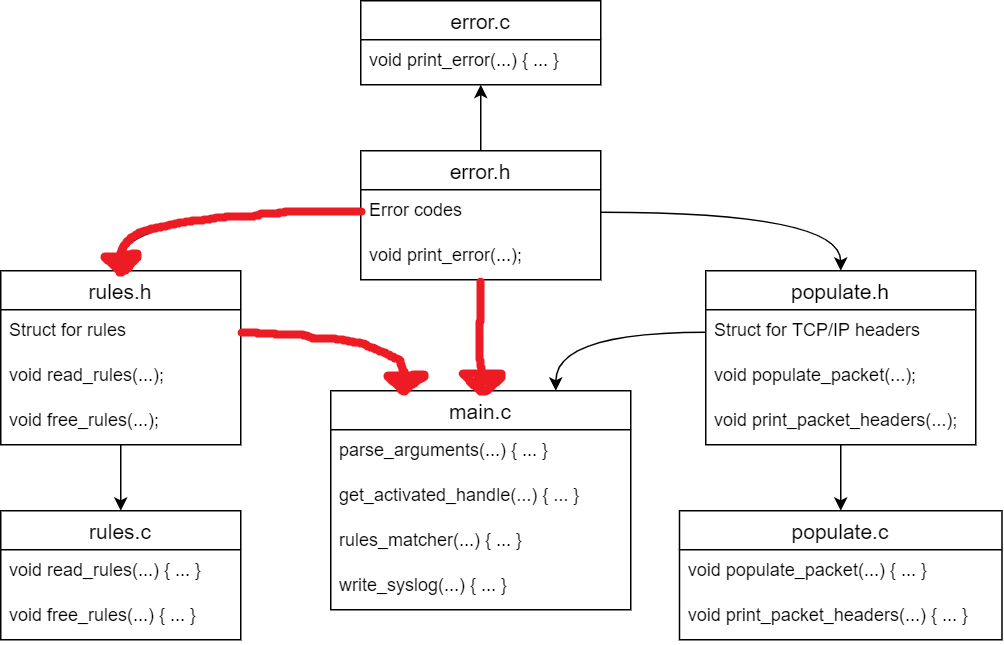
\includegraphics[width=0.80\linewidth]{images/double-include.png}
    \caption{Illustration de la double inclusion}
    \label{fig:doubleinclusion}
\end{figure}










\section{Améliorations possibles}





\subsection{Changement au niveau des règles ou du fichier de règles}



\begin{itemize}
    \item Prendre en charge les adresses des protocoles IPv6 et Ethernet au niveau des règles.
    \begin{example}
        Pour le moment, seules les adresses IPv4 peuvent être traitées par l'IDS. Comme la longueur et le format des adresses de ces trois protocoles (IPv4, IPv6, Ethernet) sont forts différents, on pourrait faire une fonction qui vérifie le format d'adresse utilisé (donc pas besoin que l'utilisateur précise le protocole lui-même).

        Il faudrait aussi changer le code dans la fonction \textit{read\_rules} pour prendre en charge ces autres types d'adresses.
    \end{example}
    \item Pouvoir écrire un message d'erreur qui précise aussi les numéros de ligne et colonne quand il y a un problème.
    \begin{example}
        Il faudrait pouvoir écrire des message d'erreur quand le fichier ids.rules contient des erreurs. Par exemple, si il manque une virgule, une parenthèse fermante, etc. J'ai ajouté la figure \ref{fig:exerreur} pour avoir un exemple de bon message d'erreur. Il montre les numéros de ligne et colonne, il affiche  le contenu des lignes entourant l'erreur, et explique ce que le compilateur attendait.
        \begin{figure}[H]
            \centering
            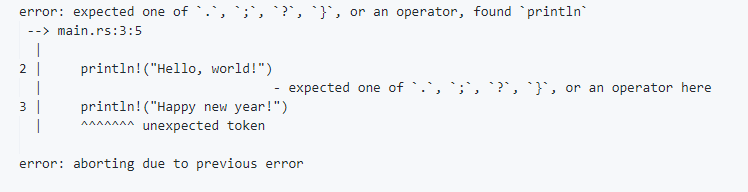
\includegraphics[width=0.90\linewidth]{images/exemple-erreur.PNG}
            \caption{Exemple de message d'erreur}
            \label{fig:exerreur}
        \end{figure}
    \end{example}
    \item Ajouter la possibilité d'écrire des commentaires dans le fichier de règles.
    \begin{example}
        Ce serait bien de pouvoir écrire des commentaires qui expliquent une règle. Par exemple, si on croise un \# dans le fichier de règles, le reste de la ligne est ignoré par la fonction \textit{tokenize\_rules}. Le problème vient évidemmment du fait qu'un utilisateur de l'IDS peut vouloir utiliser un \# dans l'option \textit{content} d'une règle pour vérifier que certains paquets ne continennent pas ce caractère. Il faut donc ajouter une possibilité d'échappement.
    \end{example}
\end{itemize}





\subsection{Prise en charge de plus d'actions}



\begin{itemize}
    \item Prendre en charge l'action \textit{drop} pour pouvoir laisser tomber un paquet sans qu'il puisse être utilisé par d'autres programmes.
    \begin{example}
        On pourrait créer des \textit{iptables} pour envoyer les paquets dans une file pour les analyser et décider si on les laisse tomber ou pas, et ce avant qu'ils ne soient analysés \cite{12}.
    \end{example}
    \item Prendre en charge l'action \textit{reject} qui \textit{drop} le paquet puis envoie un message "RST/ICMP unreach error".
    \item Ajouter une option pour que notre IDS fasse l'équivalent d'une attaque \textit{man in the middle} (mais légitime) afin d'analyser le contenu des paquets cryptés.
    \begin{example}
        Certaines organisations ont une politique de sécurité informatique telle que les données cryptées doivent être décryptées puis analysées avant d'être éventuellement ré-encryptées \cite{13}. Ceci est illustré par la figure \ref{fig:tlsanalysis}.
        \begin{figure}[H]
            \centering
            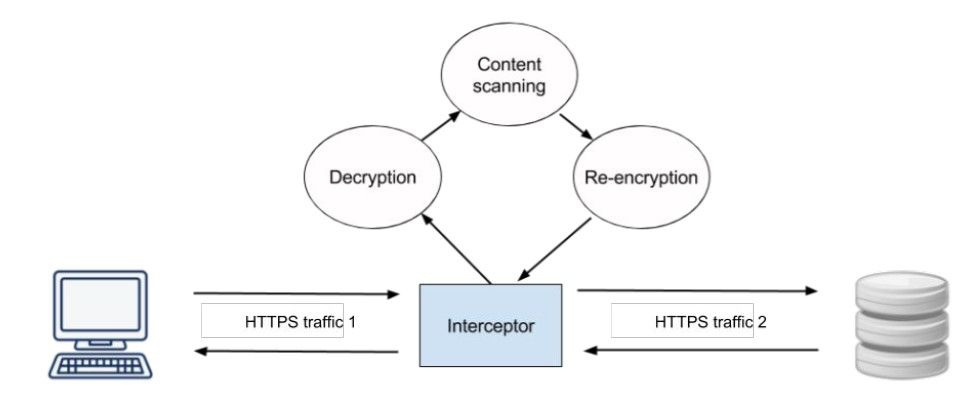
\includegraphics[width=0.99\linewidth]{images/tls-analysis.jpg}
            \caption{Analyse TLS \cite{13}}
            \label{fig:tlsanalysis}
        \end{figure}
    \end{example}
\end{itemize}





\subsection{Autres améliorations}



\begin{itemize}
    \item Afficher une erreur quand les arguments donnés à l'IDS en ligne de commande sont incorrects.
    \begin{example}
        Pour le moment, si un mauvais argument est donné à l'IDS, il est simplement ignoré. Ce serait mieux d'afficher un message d'erreur qui aide l'utilisateur à corriger son erreur.
    \end{example}
    \item Ajouter des fichiers pour simplifier l'organisation du code.
    \begin{example}
        Le nombre de lignes de code et de fonctions est plutôt élevé. Le projet gagnerait en simplicité si certaines fonctions, structures ou enums étaient placées dans d'autres fichiers. Par exemple, nous utilisons deux enums pour les protocoles (\textit{RuleProtocol} et \textit{PopulateProtocol}). Notre base de code serait simplifiée si on n'en utilisait qu'une, en la mettant dans un fichier header \textit{protocol.h}.
    \end{example}
\end{itemize}










\section{Conclusion}



Nous avons beaucoup appris avec ce projet, en particulier quand nous avons essayé de résoudre les problèmes rencontrés. Par exemple, nous savons maintenant comment gérer des structures de données dynamiques, travailler avec du binaire (shift, et/ou logique), utiliser des include guards, etc. Mais en-dehors de la programmation elle-même, nous avons appris beaucoup dans des sujets traités par le projet, comme l'utilisation des headers des protocoles réseau et leur analyse en sécurité informatique. En conclusion, nous avons appris comment les IDS fonctionnent et nous en avons implémenté un simplifié.















\newpage \tableofcontents \listoffigures
\begin{thebibliography}{9}
\bibitem{1} {\small \url{https://github.com/groumache/Intrusion-Detection-System}}
\bibitem{2} {\small \url{https://suricata.readthedocs.io/en/latest/rules/intro.html}}
\bibitem{3} {\small \url{https://qr.ae/pNSWwR}}
\bibitem{4} {\small \url{https://stackoverflow.com/a/16268404/10524378}}
\bibitem{5} {\small \url{https://fr.wikipedia.org/wiki/Liste_de_ports_logiciels}}
\bibitem{6} {\small \url{https://www.seas.upenn.edu/~cis522/lecture_notes/lec11.pdf}}
\bibitem{7} {\small \url{https://uynguyen.github.io/2018/04/30/Big-Endian-vs-Little-Endian/}}
\bibitem{8} {\small \url{https://gcc.gnu.org/onlinedocs/gcc-3.2/gcc/Variable-Attributes.html}}
\bibitem{9} {\small \url{https://stackoverflow.com/a/45433017/10524378}}
\bibitem{10} {\small \url{https://gcc.gnu.org/onlinedocs/cpp/Pragmas.html}}
\bibitem{11} {\small \url{https://fr.wikipedia.org/wiki/Include_guard}}
\bibitem{12} {\small \url{https://www.linuxquestions.org/questions/linux-networking-3/capture-drop-packets-using-c-716868/#post3498563}}
\bibitem{13} {\small \url{https://qr.ae/pNJyLS}}
\end{thebibliography}




















\end{document}
